\begin{houseviewbox}[核心结论]
本报告的核心不是列出“华为超节点概念股”，而是回答三个问题：\textbf{实物展示究竟验证了什么、哪些上市公司拥有可核验关系、当前价格是否留下安全边际。}截至 2026 年 7 月 18 日，华为官方证据确认 1,024 卡 Atlas 950 实物系统已公开展示，FP8/FP4 标称算力分别为 1/2 EFLOPS，提供 256TB 全局统一地址空间、TB 级 NPU 互联与 3 微秒往返时延；8,192 卡、128 个计算柜加 32 个互联柜仍属于 2026Q4 最大设计路线图。二者不能混写为“8,192 卡已交付”。

上市公司证据呈现明显错位：申菱环境披露华为为数据服务客户、与 H 公司合作并给出数据服务收入和订单增长；科大讯飞披露与华为围绕昇腾 950 协同并计划 2026 年 10 月发布旗舰模型；拓维信息披露昇腾系统伙伴关系及较高华为购销占比。上述证据能确认客户或生态关系，却都没有给出 Atlas 950 平台认证、订单金额、交付数量、ASP、收入确认或毛利率。因此，\textbf{本报告没有“已确认 Atlas 950 上游核心供应商”，也不把任何通用 AI 产品能力写成专属供货。}

估值结果同样不支持事件驱动追高。12 个完整模型以现股本重算 2026E/2027E EPS，主方法使用去除未桥接成长溢价后的成熟业务 PE，独立锚使用交易所年报净资产与标准化 ROE 推导的合理 P/B。沃尔核材仅剩约 +1.4\%的边际空间，其余 11 家均为负；关系更强的申菱环境和科大讯飞分别约为 -63.8\%、-61.1\%。当前没有同时满足“高关联、完整盈利桥、显著安全边际”的公司，最优策略是等待一级证据与价格重置。
\end{houseviewbox}

\begin{figure}[htbp]
\centering
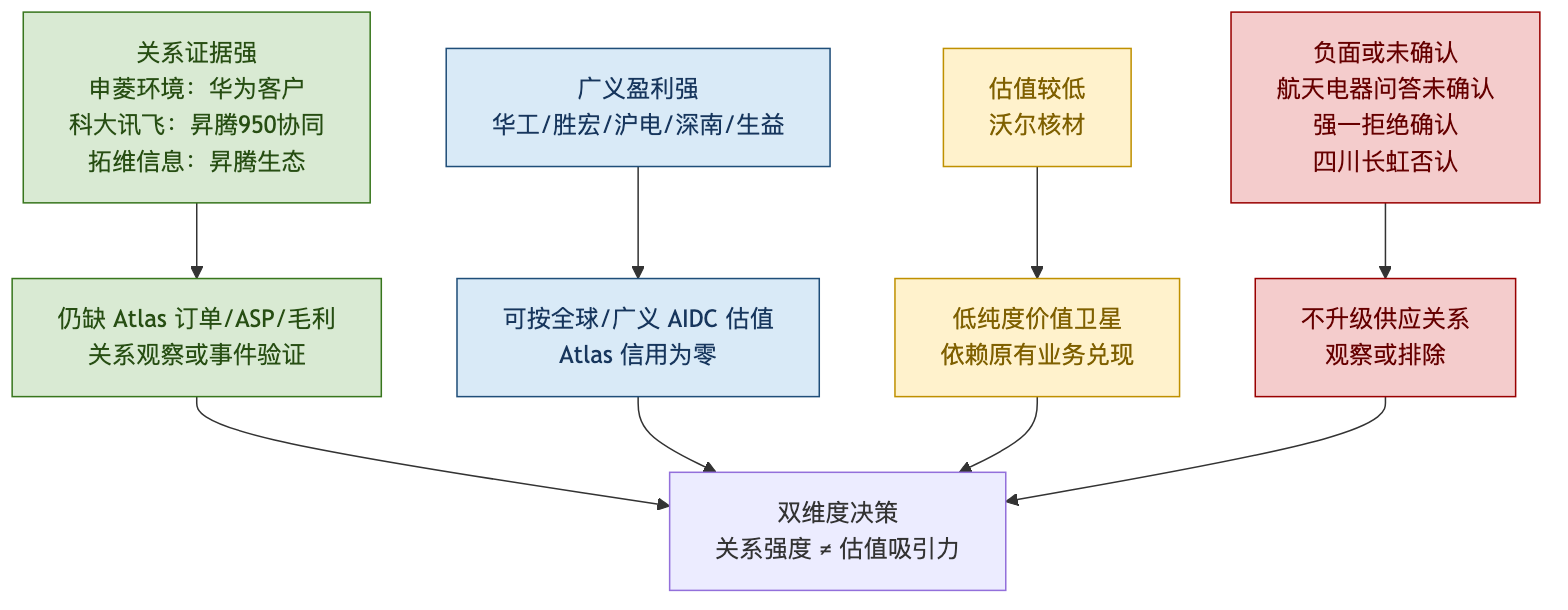
\includegraphics[width=\textwidth]{exhibits/evidence_action_map.png}
\caption{关系证据、广义盈利与估值吸引力的双维度决策}
\sourcenote{公司年报、客户链审计和现价估值模型。图中分类是研究动作，不是已确认 Atlas 供货或交易指令。}
\end{figure}

图中四组不能按一个“华为链纯度”排序：关系强的一组仍缺订单和经济性；盈利强的一组可按广义 AI 业务估值，却没有 Atlas 分配；估值较低的一组必须依赖原有业务兑现；负面/未确认组不能因产品能力被升级。这个双维度框架是后续所有动作标签的统一口径。

\begin{riskbox}[结论等级]
产业趋势：\textbf{正面}；1,024 卡实物验证：\textbf{中高置信度}；8,192 卡 2026Q4 交付：\textbf{前瞻路线图}；A 股 Atlas 专属订单：\textbf{未确认}；现阶段板块性追涨吸引力：\textbf{偏低}。报告不发布“买入”评级，只给出关系验证、价值观察和高估值风险三类跟踪动作。
\end{riskbox}

\begin{exhibitbox}[投资委员会分层表]
\begin{longtable}{L{1.5cm}L{2.1cm}L{3.5cm}R{1.5cm}R{1.5cm}R{1.5cm}L{2.2cm}}
\toprule
\textbf{代码} & \textbf{公司} & \textbf{证据定位} & \textbf{现价} & \textbf{目标} & \textbf{空间} & \textbf{动作}\\
\midrule
\endhead
301018 & 申菱环境 & 华为客户、H 公司合作；无 Atlas 订单 & 86.96 & 31.50 & -63.8\% & 最高关联观察\\
002230 & 科大讯飞 & 昇腾 950 模型协同；下游需求锚 & 41.12 & 16.01 & -61.1\% & 事件验证\\
002261 & 拓维信息 & 昇腾生态与华为购销；经常性利润弱 & 27.38 & -- & -- & 只观察、不估值\\
002130 & 沃尔核材 & 高速铜连接能力；Atlas 关系未确认 & 15.24 & 15.45 & +1.4\% & 低纯度价值卫星\\
002335 & 科华数据 & 智算供电/POD；曾服务昇腾创新中心 & 29.75 & 15.18 & -49.0\% & 等待估值回落\\
300476 & 胜宏科技 & AI PCB 高增长；Atlas 平台未确认 & 241.50 & 152.22 & -37.0\% & 选择性观察\\
000988 & 华工科技 & 800G/1.6T/3.2T 光连接能力 & 117.62 & 55.48 & -52.8\% & 等待平台订单\\
002837 & 英维克 & 端到端液冷；无华为 Atlas 分配 & 61.57 & 23.64 & -61.6\% & 等待 Q2 毛利\\
600183 & 生益科技 & AI CCL 景气；Atlas 材料规格未知 & 132.29 & 68.85 & -48.0\% & 高估值风险\\
002916 & 深南电路 & AI PCB/封装；Atlas 认证未知 & 334.00 & 201.21 & -39.8\% & 回调验证\\
002463 & 沪电股份 & AI 服务器/交换机 PCB；低专属性 & 127.80 & 61.99 & -51.5\% & 回调验证\\
002025 & 航天电器 & 背板/液冷连接器能力；问答未确认 & 64.76 & 42.06 & -35.1\% & 关系未确认观察\\
\bottomrule
\end{longtable}
\sourcenote{2026-07-17 收盘价、12 家交易所年报原件、公司问答与 38 份原始卖方 PDF。目标价只评价公司更广义业务，Atlas 专属收入信用为 0。}
\end{exhibitbox}

\begin{exhibitbox}[前三类优先标的的量化盈利门槛]
\begin{tabularx}{\textwidth}{L{2.1cm}R{1.8cm}R{1.7cm}R{1.5cm}X}
\toprule
\textbf{公司} & \textbf{2026E 收入} & \textbf{2026E 归母} & \textbf{2026E EPS} & \textbf{下一披露升级/下调阈值}\\
\midrule
申菱环境 & 67.50 & 4.28 & 1.144 & 维持全年预测且数据服务订单转收入、毛利和现金不恶化；任一全年核心预测下修超过 10\%即下调\\
沃尔核材 & 121.50 & 18.80 & 1.343 & 维持全年预测且高速线缆认证、利用率和铜价传导兑现；任一全年核心预测下修超过 10\%即移除正空间\\
胜宏科技 & 325.52 & 88.98 & 9.054 & 维持全年预测且海外产能良率、AI 产品结构和现金兑现；任一全年核心预测下修超过 10\%即下调\\
\bottomrule
\end{tabularx}
\sourcenote{单位：亿元、元。数值来自原始卖方全年预测并按现股本复算 EPS；因缺少一致的季度分部预测，本表不机械四等分，而以“全年预测变化超过 10\%”作为下一披露的可复算门槛。}
\end{exhibitbox}

\section{排序方法、收益归因与监测纪律}

投资委员会排序不使用单一“华为链纯度”，而使用四项权重：关系/来源证据 35\%、独立盈利与估值 35\%、下一季度可验证性 20\%、现金流与集中度风险 10\%。关系分决定研究优先级，估值分决定是否存在安全边际；二者不能互相替代。由于未获得用户组合、授权与流动性约束，本报告不给仓位或交易指令，以监测频率作为风险预算等价物。

\begin{exhibitbox}[前三类研究优先级与预期收益归因]
\begin{tabularx}{\textwidth}{L{2.2cm}L{2.2cm}L{3.0cm}L{3.3cm}X}
\toprule
\textbf{公司} & \textbf{目标/空间} & \textbf{收益归因} & \textbf{下一验证} & \textbf{监测预算与纪律}\\
\midrule
申菱环境 & 31.50/-63.8\% & 关系证据最强，但成熟业务 PE 与合理 P/B 均不支持现价；Atlas 贡献为 0 & 数据服务订单转收入、毛利、应收与平台点名 & 高优先级证据监测；只在订单+经济性同时出现时升级，利润/现金恶化则下调\\
沃尔核材 & 15.45/+1.4\% & 唯一微弱正空间来自原有业务与高速铜连接；Atlas 贡献为 0 & 高速线缆资格、产能利用率、铜价传导与利润 & 中优先级价值监测；安全边际不足，任一核心预测下修即移除正空间\\
胜宏科技 & 152.22/-37.0\% & 全球 AI PCB 盈利高增，但移除未桥接成长溢价后无安全边际；Atlas 贡献为 0 & 海外产能良率、AI 产品结构、毛利与现金 & 中高优先级盈利监测；增长或良率低于阈值即下调，华为订单仅为额外期权\\
\bottomrule
\end{tabularx}
\sourcenote{关系/估值/验证/风险权重分别为 35\%/35\%/20\%/10\%；价格日 2026-07-17。}
\end{exhibitbox}

除沃尔核材仅约 +1.4\% 外，其余 11 家均为负目标空间；拓维信息另因新鲜外部预测门槛未过而不发布目标价。不因一日大跌自动升级。研究动作只有四种：新增一级证据与盈利桥同时成立才“升级”；仅能力/一般关系维持“观察”；盈利、现金或路线图低于阈值则“下调”；官方否认、关系长期无证据或独立业务失去估值支撑则“移除”。

\section{四个必须分开的概念}

第一，\textbf{昇腾 950DT}是计划于 2026Q4 可用的训练/解码芯片路线图，华为披露单卡 144GB HiZQ 2.0 HBM、4TB/s 存储带宽、2TB/s 互联带宽以及 1PFLOPS FP8、2PFLOPS FP4。第二，\textbf{Atlas 950 SuperPoD}是基于 UnifiedBus 2.0 的单逻辑机系统，1,024 卡实物展示和 8,192 卡最大设计是两个状态。第三，\textbf{Atlas 950 SuperCluster}是 64 个 SuperPoD 的 scale-out 层，超过 52 万卡，不能写成一个单体超节点。第四，\textbf{A 股供应链映射}只是能力与关系审计，必须经过产品、认证/订单、交付、收入和利润五级门槛后才能进入估值。

这四层一旦混合，最常见的错误就会出现：把 256TB 全局地址空间写成 256TB HBM；把 8,192 卡路线图写成当前交付；把华为客户关系写成 Atlas 950 订单；把全球 AI 业务写成华为收入；最后再用高景气行业倍数为未经验证的专属收入定价。本报告所有模型都反向约束这些错误。

\section{三条可执行结论}

\textbf{其一，跟踪“证据升级”而不是发布会热度。}最有价值的下一条信息不是更多峰值算力数字，而是 8,192 卡实物/客户验收、950DT 量产配置、系统功耗和 BOM、公开客户与站点、上市公司平台认证与订单。只有公司公告能把能力映射升级为盈利信用。

\textbf{其二，关系强度与估值吸引力分开。}申菱环境、科大讯飞、拓维信息的关系证据更强，但财务兑现、估值或收入纯度并不同时占优；沃尔核材在保守模型中仅剩微弱正空间，科华数据和胜宏科技也已为负空间，三者均缺少 Atlas 专属证据。组合研究不能用一个“纯度分数”替代这两个维度。

\textbf{其三，2026Q4 是路线图验证窗，不是自动收入确认日。}芯片可用、系统交付、客户验收、供应商确认和上市公司收入确认之间可能跨越多个季度。若市场在第一步就一次性定价第五步，风险收益比会恶化。
